\documentclass{article}
\usepackage{graphicx}
\usepackage{amsmath}
\usepackage{pgfplots}
\usepackage{physics}
\usepackage{cancel}
\usepackage{enumitem}
\usepackage{txfonts}

\pgfplotsset{compat=1.18}

\newcommand{\Eth}{E_{\text{th}}}

\usepackage[a4paper, top=1cm, bottom=2cm, left=2cm, right=2cm, includehead, includefoot]{geometry}

\begin{document}

\noindent
Physics 4A - Classical Mechanics \hfill Prof. Roger King

\noindent\rule{\textwidth}{0.4pt}

\begin{center}
    \textbf{\LARGE Homework 13} \\
    \vspace{12pt}
    \large Aaron W. Tarajos \\
    \textit{\today}
\end{center}

\noindent\rule{\textwidth}{0.4pt}

\section*{Problem 1}
The figure below shows three 0.0100 kg particles that have been glued to a rod of length L = 6.00
cm and negligible mass. The assembly can rotate around a perpendicular axis through point $O$ at
the left end. If we remove one particle (that is, 33\% of the mass), by what percentage does the
rotational inertia of the assembly around the rotation axis decrease when that removed particle
is (a) the innermost one and (b) the outermost one?

\begin{figure}[ht]
    \centering
    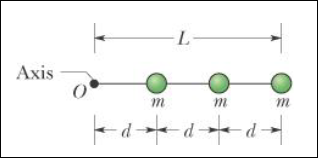
\includegraphics[scale=0.5]{drawing-1.png}
\end{figure}

\subsection*{Solution}
\subsubsection*{Part a:}
Each $I_i$ is given by
\[
	r_i^2 m_i
\]
and the total rotational inertia is the sum of all $I_i$ and the percentage change $P_I$ is given by the difference quotient before and after the masses are removed therefore we have.
\begin{align*}
	P_I &= \frac{m(r_2^2 + r_3^2) - m(r_1^2 + r_2^2 + r_3^2)}{m(r_1^2 + r_2^2 + r_3^2)} \cdot 100\\
	    &= \frac{0.0100(4^2 + 6^2) - 0.0100(2^2 + 4^2 + 6^2)}{0.0100(2^2 + 4^2 + 6^2)} \cdot 100 \\
	    &= \boxed{-7.143\ \%}
\end{align*}

\subsubsection*{Part b:}
We do the same thing removing the other mass;
\begin{align*}
	P_I &= \frac{m(r_1^2 + r_2^2) - m(r_1^2 + r_2^2 + r_3^2)}{m(r_1^2 + r_2^2 + r_3^2)} \cdot 100\\
	    &= \frac{0.0100(2^2 + 4^2) - 0.0100(2^2 + 4^2 + 6^2)}{0.0100(2^2 + 4^2 + 6^2)} \cdot 100 \\
	    &= \boxed{-64.286\ \%}
\end{align*}


\section*{Problem 2}
Two particles with masses 2.00 and 5.00 kg are connected by a light rod of length 2.00 m.
Find the moment of inertia of the system about an axis perpendicular to the rod and passing
through (a) the midpoint and (b) the center of mass.

\subsection*{Solution}
\subsubsection*{Part a:}
The rotational inertia for a rod with two particles around the midpoint is given by;
\begin{align*}
	I &= m_1 \left( \frac{1}{2}L \right)^2 + m_2 \left( \frac{1}{2}L \right)^2 \\
	  &= \frac{1}{4}L^2 \left(m_1 + m_2 \right) \\
	  &= \frac{1}{4}2.00^2 \left(2.00 + 5.00 \right) \\
	  &= \boxed{7\ \text{kg} \cdot \text{m}^2}
\end{align*}

\subsubsection*{Part b:}
Then we just have to change the radius to accomodate the respective center of mass. Let the midpoint be $x=0$ then the center of mass is;
\[
	x_{cm} = \frac{-1.0 \cdot 2.00}{7.00} + \frac{1.0 \cdot 5.00}{7.00} = 0.429\ \text{m}
\]
so our rotational intertial becomes;
\begin{align*}
	I &= 2.00 \left( 1.429 \right)^2 + 5.00 \left( 0.571 \right)^2 \\
	  &= \boxed{5.714\ \text{kg} \cdot \text{m}^2}
\end{align*}


\section*{Problem 3}
For each of the forces depicted in the figure find the torque about the pivot (black dot at
center of rod). Take $F_1 = 10.0$ N, $F_2 = 15.0$ N, $F_3 = 8.00$ N, and $L = 9.00$ m. The rods length
is $L$.

\begin{figure}[ht]
    \centering
    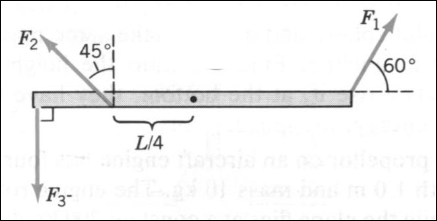
\includegraphics[scale=0.5]{drawing-2.png}
\end{figure}

\subsection*{Solution}
The torque $\tau$ is given by

\[
	\tau = rF_t\sin \phi
\]
For $\vec{F}_1$ that is;
\[
	\tau = \frac{9}{2}(10.0)\sin(60) = \boxed{38.971\ \text{N}\cdot\text{m}}
\]
for $\vec{F}_2$;
\[
	\tau = \frac{9}{4}(15.0)\sin(135) = \boxed{23.865\ \text{N}\cdot\text{m}}
\]
and for $\vec{F}_3$ that is;
\[
	\tau = \frac{9}{2}(8.00)\sin(-90) = \boxed{-36\ \text{N}\cdot\text{m}}
\]

\section*{Problem 4}
The angular position of a line on a disk of radius $r = 6.00$ cm is given by
\[
	\theta = 10.0 - 5.00 t + 4t^2 \quad \text{rad}
\]
Find: (a) the average angular speed between 1.00 and 3.00 s; (b) the linear speed of a point on
the rim at 2.00 s; (c) the radial and tangential accelerations of a point on the rim at 2.00 s.

\subsection*{Solution}
\subsubsection*{Part a:}
The average speed is given by;
\[
	\omega_\text{avg} = \frac{\theta -\theta_0}{\Delta t}
\]
$\theta$ is
\[
	10.0 - 5.0(3.0) + 4 (3.0)^2 = 31.0\ \text{rad}
\]
and $\theta_0$ is;
\[
	10.0 - 5.0(1.0) + 4(1.0)^2 = 9.0\ \text{rad}
\]

So we have
\[
	\omega_\text{avg} = \frac{31.0-9.0}{2} = \boxed{11\ \text{s}^{-1}}
\]

\subsubsection*{Part b:}
The angular velocity at time $t$ is;
\[
	\omega = \frac{d\theta}{dt} = 8t - 5.00
\]
so at 2.00 s that is;
\[
	\omega = 8(2)-5.00 = 11.0\ \text{rad}/\text{s}
\]
which we use to find the tangential velocity of;
\[
	v_t = r \omega = 6.00 \cdot 11.0 = \boxed{66\ \text{cm}/\text{s}}
\]

\subsubsection*{Part c:}
We find the angular acceleration as;
\[
	\alpha = \frac{d^2\theta}{dt^2} = 8
\]
and use that to find the tangential acceleration as;
\[
	a_r = r \alpha = 6.00 \cdot 8 = \boxed{48.00\ \text{cm}/\text{s}^2}
\]
and then radial acceleration is;

\[
	r\omega^2 = 6.00 \cdot 11.0^2 = \boxed{726\ \text{cm}/\text{s}^2}
\]

\pagebreak

\section*{Problem 5}
The book in the figure has the same shape as your physics textbook. About which axis is the
rotational inertia (a) the largest; (b) the smallest? You must justify your answer.

\begin{figure}[ht]
    \centering
    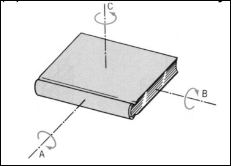
\includegraphics[scale=0.5]{drawing-3.png}
\end{figure}

\subsection*{Solution}
\subsubsection*{Part a:}
C is the axis with the largest rotational inertia because it does not rotate along the smallest dimension of the book, the spine.

\subsubsection*{Part b:}
B is the axis with the smallest rotational inertia because it is rotating about the two smallest dimensions, the spine and the width.

\section*{Problem 6}
The wheel shown in the figure below has a central hub of radius 2.00 m and a mass of 2.00
kg. Each of the four spokes is 4.00 m long and has a mass of 1.00 kg. The outer thin ring has a
radius of 6.00 m and a mass of 2.00 kg. Find the rotational inertia about an axis through the
center perpendicular to the plane of the wheel. Treat the hub as a disk. Hint, you will have to
use the parallel axis theorem with the spokes.

\begin{figure}[ht]
    \centering
    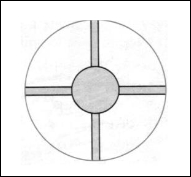
\includegraphics[scale=0.5]{drawing-4.png}
\end{figure}

\subsection*{Solution}
The total rotational inertia is the some of the rotational inertia of each component;
\[
	I = I_h + I_r + 4I_s
\]
where the subscripts $h$, $r$, and $s$ represent the hub, ring, and spokes respectively. Then
\begin{align*}
	I_h &= \frac{1}{2}mR^2 \\
	I_r &= mR^2 \\
	I_s &= \left(\frac{1}{12}mL^2\right) + m\left(\frac{L}{2}+r_h\right)^2
\end{align*}
and so we have;
\begin{align*}
	I &= \frac{1}{2}m_h R_h^2 + m_r R_r^2 + 4\left(\left(\frac{1}{12}m_s L^2\right) + m_s\left(\frac{L}{2}+r_h\right)^2\right) \\
	  &= \frac{1}{2}(2.00)(2.00)^2 + (2.00)(6.00)^2 + 4\left(\left(\frac{1}{12}(1.00)(4.00)^2\right) + (1.00)\left(\frac{4.00}{2}+2.00\right)^2\right)\\
	  &= \boxed{145.333\ \text{kg} \cdot \text{m}^2}
\end{align*}


\section*{Problem 7}
Two solid spheres of mass m and radius $R$ are stuck to the ends of a thin rod of mass $m$ and
length $3R$. Find the rotational inertia of the system about the axis at the midpoint of the rod and
perpendicular to it, as shown in the figure below.

\begin{figure}[ht]
    \centering
    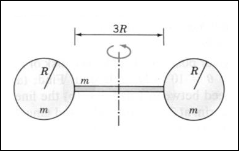
\includegraphics[scale=0.6]{drawing-5.png}
\end{figure}

\subsection*{Solution}
The total rotational inertia is the sum of the rotational of each object;
\[
	I = I_r + 2I_s
\]
where $r$ is the inertia of the rod and $s$ is the inertia of one of the spheres. Then
\begin{align*}
	I &= \frac{1}{12}m9R^2 + 2 \left( \frac{2}{5}mR^2 + m(R + 1.5R)^2 \right) \\
	  &= m \left(\frac{1}{12}9R^2 + 2 \left( \frac{2}{5}R^2 + (R + 1.5R)^2 \right)\right) \\
	  &= m \left( \frac{3}{4}R^2 + \frac{4}{5}R^2 + 12.5R^2\right) \\
	  &= \boxed{\left(\frac{31}{20}+12.5\right)mR^2}
\end{align*}

\section*{Problem 8}
A light (massless) rod of length $L = 1.5$ m is freely pivoted at one end. Three forces act as
shown in the figure below. The force $\vec{F_3}$ acts at the midpoint. What is the torque due to each force?
Take $F_1 = 6.90$ N, $F_2 = 4.00$ N, $F_3 = 2.00$ N, $\theta = 20^\circ$, and $\alpha = 30^\circ$

\begin{figure}[ht]
    \centering
    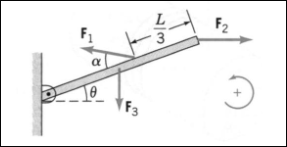
\includegraphics[scale=0.6]{drawing-6.png}
\end{figure}


\subsection*{Solution}
We solve for the torque in the same manner as problem 3;
\begin{align*}
	\vec{F}_1 r \sin \phi &= 6.90 \cdot \frac{2}{3}1.5 \cdot \sin(30) = \boxed{3.45\ \text{N}\cdot\text{m}} \\
	\vec{F}_2 r \sin \phi &= 4.00 \cdot 1.5 \cdot \sin(-20) = \boxed{-2.052\ \text{N}\cdot\text{m}} \\
	\vec{F}_3 r \sin \phi &= 2.00 \cdot 0.75 \cdot \sin(-70) = \boxed{-1.410\ \text{N}\cdot\text{m}} \\
\end{align*}

\end{document}
